\section{OD data preparation and correction of simulations}

\subsection{OD Energy Scale} \label{sec:od_energy_scale}
\par
After construction and filling of the OD, the single photoelectron response for each PMT was determined using the OD optical calibration system (OCS) \cite{lz_ocs_system_ref}.
A detailed description of the PMT monitoring during commissioning and the first science run (SR1) can be found in the works of E. Fraser \cite{ewanfraser_thesis_ref}. 
During this period, an energy calibration of the OD was also performed.
Again, details of the methodology are the work of E. Fraser \cite{ewanfraser_thesis_ref} but summarised below, as the result is used throughout this chapter.
\par
For the energy calibration, 7 $\gamma$ sources were used which are summarised in \autoref{tab:od_energy_calibration_sources}.
Each were lowered into a single CSD to the 700 mm level (see \autoref{fig:CSD1_Geometry}).
The signals from these $\gamma$s were picked out giving 7 data points for a conversion between signal size and $\gamma$ energy.
As discussed in \autoref{sec:od_physics}, there is a non-linear energy response in the scintillator, and therefore a non-linear energy scale below 300 keV.
The empirical formula which describes this non-linearity, developed by DayaBay \cite{dayabay_antineutrino_oscillation_ref, ls_nonlinear_energy_response_ref}, is given by:
\begin{equation}
    \frac{E_{vis}}{E_{true}} = \frac{p_0  + p_3 \times E_{true}}{1 + p_1 \times e^{p_2 \times E_{true}}}
    \label{eq:ls_light_response}
\end{equation}
where $E_{true}$ is a amount of energy deposited, $E_{vis}$ is the amount of energy observed and $p_0$, $p_1$ and $p_3$ are constants.

\par
\autoref{eq:ls_light_response} was used to fit the 7 data points which is shown in \autoref{fig:od_energy_scale}.
This then gives a translation from signal size to energy for any signal, and importantly for the OD veto, a value in photons detected (phd) for 100 keV and 200 keV events.
The amount of light observed by the LZ OD is in line with other LAB-based experiments as can be seen in \autoref{tab:od_phe_per_mev_comparison}.
\begin{table}[]%
    \centering
    \begin{tabular}{c|c|c}
        Source      & Specific observable         &  $\gamma$ energy (keV) \\ \hline
        ${}^{57}Co$ & direct $\gamma$             & 122                        \\
        ${}^{22}Na$ & positron annihilation       & 511               \\
        ${}^{54}Mn$ & direct $\gamma$             & 835                        \\
        ${}^{22}Na$ & direct $\gamma$             & 1275               \\
        ${}^{252}Cf$ & neutron capture on H       & 2223            \\
        ${}^{228}Th$ & ${}^{208}Tl$ $\beta-$decay & 2615            \\
        ${}^{252}Cf$ & neutron capture on Gd      & 8000            
        
    \end{tabular}
    \caption{Calibration sources used to determine the OD energy scale.}
    \label{tab:od_energy_calibration_sources}
\end{table}

\begin{figure}[]
    \centering
   \begin{tikzpicture}
    \begin{groupplot}[%view={0}{90},
    group style = {group size = 1 by 2,vertical sep=0.5cm},
                   width=0.98\textwidth]
    \nextgroupplot[
            ylabel=LS energy response ($\frac{E_{vis}}{E_{true}}$),
            %xlabel=,
            xticklabels={,,}
            height=10cm, width=\textwidth,
            xmin=0, xmax=10,
            grid=major,
            ]
            %\addplot[black, smooth, domain=0:10] 
                    %{(0.00535 + 0.0286*x) / (1-0.9918*exp(-0.03018*x))};
                    %{((0.001894 + 0.03614*x) / (1-1*exp(-0.001453*x)))};
            \addplot[black, smooth]
                table[x=Energy,y=Value]
                {Data/OD_Energy_Scale/emperical_fit.dat};
                    
            \addplot[only marks,
                 error bars/.cd,
                 y dir=both, y explicit, error bar style={color=black}] table[x=Energy,y=light_response, y error=light_response_Error] {Data/OD_Energy_Scale/phd_energy.dat};

    \nextgroupplot[
            ylabel=N. photons detected,
            xlabel=Energy (MeV),
            height=6cm, width=\textwidth,
            xmin=0, xmax=10,
            ymin=0, 
            grid=major,
            ]
            \addplot[only marks,
                 error bars/.cd,
                 y dir=both, y explicit, error bar style={color=black}] table[x=Energy,y=pulseArea, y error=pulseArea_Error] {Data/OD_Energy_Scale/phd_energy.dat};
            \addplot[black, smooth, domain=0:10] 
                    {-33.98 + 0.2425*x*1000};
            
  \end{groupplot}
    \end{tikzpicture}
    \caption{OD Energy Scale and the relation between observed number of photons and the energy deposited. Analysis by E. Fraser \cite{ewanfraser_thesis_ref}.}
    \label{fig:od_energy_scale}
\end{figure}

%    \nextgroupplot[
%            ylabel=N. photons detected,
%            xlabel=Energy (MeV),
%            height=6cm, width=\textwidth,
%            xmin=0, xmax=10,
%            ymin=0, 
%            grid=major,
%            ]
%            \addplot[black]
%                    table [x=Energy,y=Value]
%                    {Data/OD_Energy_Scale/phd.dat};

\begin{table}[]%
    \centering
    \begin{tabular}{c|c}
        Detector & phe/MeV \\ \hline
        RENO     & 150 \cite{reno_phe_per_mev_ref} \\
        Borexino & 438 \cite{pablo_mosteiro_thesis_ref} \\
        Daya Bay & 162 \cite{dayabay_phe_per_mev_ref} \\
        Kamland  & 200 \cite{kamland_phe_per_mev_ref} \\
        SNO+     & 300 \cite{snoplus_phe_per_mev_ref} \\
        LZ       & 230 
    \end{tabular}
    \caption{LZ OD photons detected per electron equivalent MeV deposited compared to other large LAB experiments.}
    \label{tab:od_phe_per_mev_comparison}
\end{table}

\subsubsection{Energy Uncertainty}
\par
One of the largest drawbacks of the energy calibration approach used here is that only a single location was used, in detector $z$-axis.
Therefore the variation in light collection efficiency in the OD is not taken into account (see \autoref{fig:od_lce}), and so energy deposits in other locations in the GdLS would be reconstructed with incorrect energies.
This is tested in the following sections and luckily appears to be insignificant as other factors are more important.
\par
Due to error propagation from PMT single photoelectron calibrations there is $\backsim$7\% error on both the energy scale and pulse area values \cite{ewanfraser_thesis_ref}.


\subsection{PMT Noise}
\par
The waveforms from PMTs in the OD occasionally displayed erratic behaviour such as is shown in \autoref{fig:od_noise_cut_waveforms}.
This was tracked down to a grounding issue, which occasionally caused high energy pulses with large PMT multiplicities.
During this high noise period no physical OD event can be made out from the noise.
Included as well are waveforms from during a quiet period of data taking showing the regular behaviour.
\par
Within the pulse parameters it is fairly easy to pick out these noisy moments as can be seen in \autoref{fig:od_noise_cut}.
The central distribution with a pulse amplitude over pulse area of 0.01 corresponds to a regular PMT response and represents a physics signals.
There are then two other distributions.
The population with a amplitude to area pulse ratio of 0.005 are the noise events from grounding.
The other population begin above a ratio of 0.015 but as the area increases the ratio drops, until at 400 phd the ratio is zero and can originate from the same behaviour but is usually noise isolated to a single PMT.
In order to remove these pulses from any analysis, a noise cut was developed to remove these based upon the pulse shape, requiring that a large portion of the pulse integral be within 100 ns of the pulse starting.
Combined with a PMT multiplicity requirement of 5, PMT after-pulsing and dark counts are also removed.
This combined selection is used throughout this chapter being referred to as the ``noise cut".


\begin{figure}[]
\begin{subfigure}{\textwidth}
  \centering
  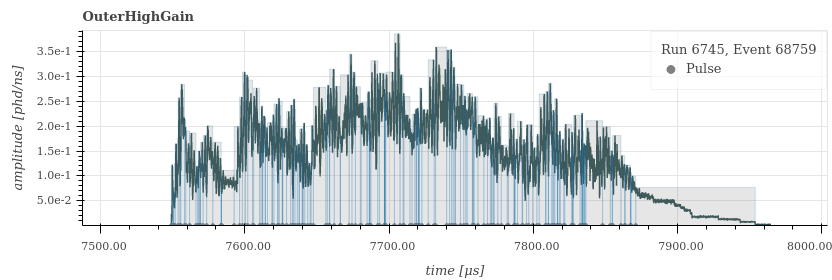
\includegraphics[width=\linewidth]{Figures/OD_Backgrounds/noise_pulse.png}
  \caption{High noise period.}
  \label{fig:noise_od_waveform}
  \end{subfigure}
  \begin{subfigure}{\textwidth}
  \centering
  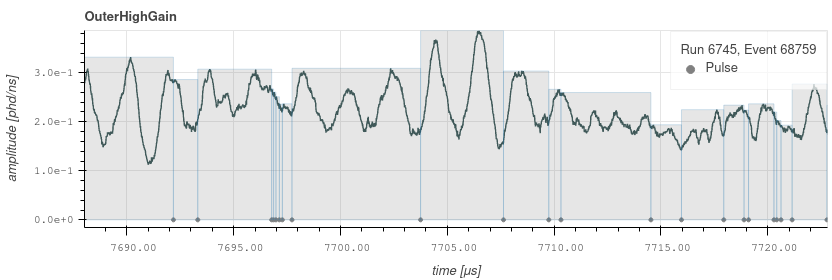
\includegraphics[width=\linewidth]{Figures/OD_Backgrounds/noise_pulse_zoomed.png}
  \caption{High noise period zoomed}
  \label{fig:noise_od_waveform_zoomed}
  \end{subfigure}
  \begin{subfigure}{\textwidth}
  \centering
  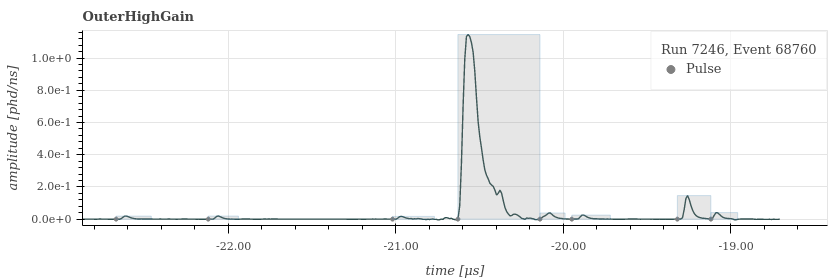
\includegraphics[width=\linewidth]{Figures/OD_Backgrounds/regular_pulse.png}
  \caption{Regular pulses}
  \label{fig:regular_od_waveform}
  \end{subfigure}
\caption{OD summed waveforms showing a noisy period of data and a regular period.}
\label{fig:od_noise_cut_waveforms}
\end{figure}


\begin{figure}[]%
\centering
\begin{tikzpicture}
\centering
  \begin{axis}[%point meta max=150,
    %point meta min=0.0,
    height=10cm, width=10cm,
    view={0}{90},
    ylabel={Pulse Amplitude/Pulse Area},
    xlabel={Pulse Area (phd)},
    xmin=0, ymin=0,
    colorbar,
    colorbar style={ylabel={Count (log$_{10}$}),},
    ]
    \addplot3[
      surf,
      shader=flat corner,
	  mesh/cols=22,
	  mesh/ordering=rowwise,
	  point meta = {z<0.1 ? nan : z}
    ] file {Data/OD_Energy_Scale/noise_cut_2d_low_2.dat};
    
    \addplot3[
      surf,
      shader=flat corner,
	  mesh/cols=30,
	  mesh/ordering=rowwise,
	  point meta = {z<0.1 ? nan : z}
    ] file {Data/OD_Energy_Scale/noise_cut_2d_high_2.dat};
\end{axis}
\end{tikzpicture}
\caption{Representative pulses seen in the OD during SR1.
         No pulse selection has been applied.
         Real events are in the distribution around 0.01 height/area.}
\label{fig:od_noise_cut}
\end{figure}

%%%%%%%%%%%%%%
\subsection{Comparison to Simulations}
\par

When data and simulations were first compared, it became obvious that the light modelling in the OD was significantly different to reality.
In \autoref{fig:od_sim_vs_data_raw} a comparison between the expected OD backgrounds and the observed background spectra are shown for two parameters: pulse area and PMT multiplicity.
The pulse area is measured in photons detected (phd) and is derived from the single photoelectron calibrations.
In the pulse area, the simulated pulse area is significantly lower than is observed in data.
Around 50\% of this difference can be accounted for by a mismatch between the PMT gains simulated against those in the reconstruction database.
This results in smaller simulated pulses but it is just a linear scaling.
However when we look at the pulse multiplicity (how many PMTs saw light in that pulse) there is also a mis-match.
This is more significant as it indicates that the light propagation within the simulation is incorrect.
In fact it would indicate that the light collection efficiency (LCE) is twice what is currently simulated (when compared to \autoref{fig:od_lce}).

\begin{figure}[]%
\centering
\begin{tikzpicture}
\centering
    \begin{groupplot}[
    group style = {group size = 1 by 2,vertical sep=2.0cm}
    ]
    \nextgroupplot[
            ylabel=Rate (Hz),
            xlabel=Pulse Area (phd),
            width=15cm,
            height=8cm,
            grid=major,
            xmin=0, xmax=700,
            ymin=1e-2, ymax=100,
            ymode=log,
            ]
        \addplot[only marks, mark size=1.0pt, error bar legend] 
            plot[error bars/.cd, x dir=both, x explicit, y dir=both, y explicit,]
            table[x=pulsearea,y=weight,x error=xerror, y error=yerror]
            {Data/OD_Backgrounds/background_constraints/od_data.dat};
        \addplot[red, const plot]
            table [x=centre,y=rate]
            {Data/OD_Backgrounds/background_fit/no_scaling/total_improved_bg_phd.dat};
        \legend{Data, Simulation};
        
            
    \nextgroupplot[
            ylabel=Rate (Hz),
            xlabel=Pulse Coincidence (PMT multiplicity),
            width=15cm,
            height=8cm,
            grid=major,
            xmin=0, xmax=120,
            %ymin=1e-2, ymax=50,
            ymode=log,
            ]
        \addplot[black, only marks, mark size=1.0pt, error bar legend,
                 error bars/.cd, error bar style={color=black},
                 y dir=both, y explicit, 
                 x dir=both, x explicit,
                 ]
            table [x=centre,y=rate,
             y error minus index=4, 
             x error minus index=6, 
            ]
            {Data/OD_Backgrounds/background_fit/no_scaling/data_bg_coincidence.dat};
        \addplot[red, const plot]
            table [x=centre,y=rate]
            {Data/OD_Backgrounds/background_fit/no_scaling/total_improved_bg_coincidence.dat};
        \legend{Data, Simulation};
    
    \end{groupplot}
\end{tikzpicture}
    \caption{Comparison of two analysis quantities; pulse area and pulse multiplicity.
             Data rates are from a single week of Random Trigger data taken during SR1.
             The simulated rates include all detector components and cavern-$\gamma$'s.}
    \label{fig:od_sim_vs_data_raw}
\end{figure}

\par
Despite this difference there are a number of ways in which data and simulations can be compared.
The simplest approach is to assume that all of the physics is correct in the simulation and the discrepancy can be accounted for entirely by an incorrect linear scaling in the simulated PMT response.
An alternative approach to compare simulations to data would be to translate phd into energy for both simulations and data, though generally the less manipulation that is performed on data the better.
Both of these approach allow for the signal sizes to be compared whilst ignoring the underlying difference in light propagation.

\par
In order to determine the factor needed to scale the simulations to observations, two reference decays were compared.
The first was from ${}^{208}$Tl which appears in the ${}^{232}$Th decay chain (shown in \autoref{fig:decay_chains}) and has a prominent 2.6 MeV $\gamma$ \cite{radon_chains_ref}.
During the OD energy calibration, ${}^{228}$Th was used (which is also part of the decay chain).
The second is from the 2.2 MeV $\alpha$-decay of ${}^{152}$Gd.
As this decay is internal to the GdLS it is spread throughout the acrylic tanks and is always present in the OD background spectrum.
As $\alpha$s are heavily quenched in the GdLS, the visible energy is in the non-linear region of the energy scale.

\par
Full-model simulations were performed of ${}^{228}$Th decays in CSD-1 at 700 mm (\autoref{fig:CSD1_Geometry}) to match the calibrations.
The 2.6 MeV $\gamma$ is the dominant decay which is able to escape the CSD and enter the OD, making it the largest feature in data.
Similarly, simulations of ${}^{152}$Gd were performed with the decays spread throughout the GdLS.
As only a single source was simulated a single peak is present in the pulse area distribution.
In data as the distribution is so low in energy is appears as a shoulder because of other backgrounds being present.
A comparison between the simulated and observed spectra for each source is shown in \autoref{fig:od_scaling_points}.
The distributions have been normalised such that the quantity of interest is at 1.

\par
The scaling factors were determined by fitting Gaussians to the pulse area distributions and dividing the Gaussian means.
Both methods provided similar, yet slightly different scaling values of 4.54 from ${}^{152}$Gd and 4.77 from ${}^{208}$Tl.
There are a number of possible reasons for this difference.
In the case of ${}^{152}$Gd, there is another $\alpha$-decaying contaminant in the GdLS: ${}^{147}$Sm \cite{scotthaselschwardt_thesis_ref}.
${}^{147}$Sm decays emitting an $\alpha$ of of 2.3 MeV, however once quenching has been taken into account the difference in the observed energy will be negligible.
The other decay limited to that region is ${}^{14}$C, a $\beta$ decay with an endpoint of 156.5 keV, overlapping with ${}^{152}$Gd.
There are also low energy cavern-$\gamma$ events which are likely to cause some spread skewing in this region.
The ${}^{152}$Gd value will also have some variation due to position, smearing out the shoulder.
Additionally as ${}^{152}$Gd appears in the non-linear response area that may also contribute to the difference as simulating the complex absorption and reemission of photons in the LS is difficult \cite{ls_nonlinear_energy_response_ref}.
%The ${}^{152}$Gd value is most likely being heavily influenced by its proximity to the high rate of very low energy events.

\par
For a full background model (described in the previous chapter), a range of scaling factors were compared against the observation.
These are shown in \autoref{fig:od_sim_vs_data_scaling_options}.
Of the four which were tried, the scaling factor of 4.54 proved to be the closest match visually via features and so was taken as the value to use.
This approach has some significant uncertainty, which will become apparent later in the next section where the backgrounds are studied.


\begin{figure}[]%
\centering
\begin{tikzpicture}
\centering
    \begin{groupplot}[
    group style = {group size = 1 by 2,vertical sep=2cm,
                   horizontal sep=0.4cm},
                   height=7cm, width=15cm
    ]
    \nextgroupplot[
            ylabel=Rate (Arb.),
            grid=major,
            xmin=0, xmax=50,
            ymin=1e-2, ymax=10,
            ymode=log,
            ]
            
        \addplot[black, only marks, mark size=1.0pt, error bar legend,
                 error bars/.cd, error bar style={color=black},
                 y dir=both, y explicit, 
                 x dir=both, x explicit,
                 ]
            table [x=pulsearea,y=weight,
            y error=yerror, x error=xerror]
            {Data/OD_Energy_Scale/gd152_data.dat};
        \addplot[red, const plot]
            table [x=pulsearea,y=weight,
            y error=yerror, x error=xerror]
            {Data/OD_Energy_Scale/gd152_sims.dat};            

        \legend{Data, Simulation};
            
    \nextgroupplot[
            ylabel=Rate (Arb.),
            xlabel=Pulse Area (phd),
            grid=major,
            xmin=0, xmax=800,
            ymin=1e-2, ymax=10,
            ymode=log,
            ]
        \addplot[black, only marks, mark size=1.0pt, error bar legend,
                 error bars/.cd, error bar style={color=black},
                 y dir=both, y explicit, 
                 x dir=both, x explicit,
                 ]
            table [x=pulsearea,y=weight,
            y error=yerror, x error=xerror]
            {Data/OD_Energy_Scale/tl208_data.dat};
        \addplot[red, const plot ]
            table [x=pulsearea,y=weight,
            y error=yerror, x error=xerror]
            {Data/OD_Energy_Scale/tl208_sims.dat};
        \legend{Data, Simulation};
    
    \end{groupplot}
\end{tikzpicture}
    \caption{Scaling points to compare simulations to observations in pulse area.
    The observed values are shown in black, and the simulation in red.
    \textbf{Top}: ${}^{152}$Gd from simulation and data.
    \textbf{Bottom}: ${}^{208}$Tl from simulation and data.
    Each distribution has been normalised to the bin of interest.}
    \label{fig:od_scaling_points}
\end{figure}

\begin{figure}[]%
\centering
\begin{tikzpicture}
\centering
    \begin{axis}[
            ylabel=Rate (Hz),
            xlabel=Pulse Area (phd),
            width=15cm,
            height=8cm,
            grid=major,
            xmin=20, xmax=700,
            ymin=1e-4, ymode=log,]
            
        \addplot[only marks, mark size=1.0pt, error bar legend] 
            plot[error bars/.cd, x dir=both, x explicit, y dir=both, y explicit]
            table[x=pulsearea,y=weight,x error=xerror, y error=yerror]
            {Data/OD_Backgrounds/background_constraints/od_data.dat};
            
        \addplot[red, const plot]
            table [x=centre,y=rate]
            {Data/OD_Backgrounds/background_fit/scaling_options/total_improved_scaling_4.37_phd.dat};
        \addplot[green, const plot]
            table [x=centre,y=rate]
            {Data/OD_Backgrounds/background_fit/scaling_options/total_improved_scaling_4.54_phd.dat};
        \addplot[blue, const plot]
            table [x=centre,y=rate]
            {Data/OD_Backgrounds/background_fit/scaling_options/total_improved_scaling_4.77_phd.dat};
        \addplot[purple, const plot]
            table [x=centre,y=rate]
            {Data/OD_Backgrounds/background_fit/scaling_options/total_improved_scaling_4.97_phd.dat};
            
        \legend{Data, 4.37 scaling, 4.54 scaling, 4.77 scaling, 4.97 scaling};
                
    \end{axis}
            
\end{tikzpicture}
    \caption{Comparison of observed and simulated pulse area distributions. 
             The simulated pulse areas have been scaled by a range of scaling values.
             The simulation distribution is from the expected rates described in \autoref{sec:simulated_od_backgrounds}.
             Both simulation and data are normalised to the same exposure.}
    \label{fig:od_sim_vs_data_scaling_options}
\end{figure}

